\documentclass[7pt]{article}

\usepackage[a4paper, total={183mm, 247mm}]{geometry}
\usepackage{hyperref}
\usepackage[utf8]{inputenc}
\usepackage{graphicx}
\usepackage{subcaption}
\usepackage{caption}
\usepackage{siunitx}
\graphicspath{{./images/}}
\usepackage{amsmath}
\usepackage{amsfonts}
\usepackage[version=4]{mhchem}
\usepackage{lineno}
\linenumbers

\newcommand*{\diff}{\mathop{}\!\mathrm{d}}
\newcommand*{\ISF}{\operatorname{ISF}}
\renewcommand*{\Re}{\operatorname{Re}}

\title{Supplemental Information}

\begin{document}

\maketitle
\tableofcontents

\section{The Langevin potential energy surface}

Attached as CSV file.

\section{Energy exchange rate of the 3D simulation}

\begin{figure*}
	\centering
	\includegraphics[width=0.5\textwidth]{MD_e_auto}
	\caption{The total energy autocorrelation function of the 3D simulation shows an extremely fast drop at short times not present in 2D simulations. This is assumed to be caused by fast motion in the perpendicular co-ordinate. To compensate for this, the decay rate of the tail is used as the energy exchange rate for this simulation.} 
	\label{fig:MD_e_auto}
\end{figure*}

There is a certain ambiguity as to what energy to use for the definition of the energy exchange rate of the 3D simulation. Although energy may be exchanged with the third co-ordinate, the motion in the this direction is generally much faster than in the lateral directions. This leads to undesirable oscillations in the total energy auto-correlation function if one tries to use a definition in terms of the lateral co-ordinates only. Subsequently, we decided to used the the sum of kinetic energy in all three dimensions and the free energy as a function of all three co-ordinates. The 3D free energy was determined in the same fashion described in the methods section except the position were binned on a 3D grid. The resulting total energy autocorrelation function, Fig. \ref{fig:MD_e_auto}, contains an extremely fast drop at short times not present in 2D simulations. This is assumed to be caused by fast motion in the perpendicular co-ordinate, but is not fully understood. To compensate for this, the decay rate of the tail is used as the energy exchange rate for this simulation. An investigation into how to rigorously define effective 2D properties from such 3D simulations is a potential avenue for future work.

\section{Derivation of the suppression factor for a particle in a harmonic well with non-Markovian noise} \label{sec:suppresion_factor}

The non-Markovian Langevin equation for a particle of mass $m$ in a harmonic well of natural frequency $\omega_0$ is given by
\begin{equation}
	m\ddot{\vec{r}}+m\eta\int\diff{t'}K(t-t')\dot{\vec{r}}(t')+m\omega_0^2\vec{r}=\vec{f}(t)
\end{equation}
\begin{equation}
	\text{ where } \left<f(t_1)f(t_2)\right>=2k_BTm\eta K(\left|t_1-t_2\right|).
\end{equation}
The memory kernel, $K(t)$, is usually assumed to be causal and have a total area of $1$. Taking the Fourier transform of this equation, applying the convolution theorem, and collecting terms results in a solution for the particle's trajectory in Fourier space in terms of a Green's function $\tilde{F}$,
\begin{equation}
	\tilde{x} = \frac{1}{m} \frac{\tilde{f}}{-\omega^2 + i \eta \omega \tilde{K} + \omega_0^2} = \frac{1}{m} \tilde{f} \tilde{F} 
	\label{eq:greens_function}
\end{equation}
\begin{equation}
	\implies x(t) = \frac{1}{m}\int\frac{\diff{\omega}}{2\pi}\tilde{f} \tilde{F} e^{i\omega t}.
\end{equation}
For the sake of clarity, we will make some reasonable claims now which will be justified in following sections. First, we claim that the ensemble average of observables like the energy exchange rate, $\phi^{-1}$, are functions of the positions of the poles of $\tilde{F}$. Furthermore, a non-constant $\tilde{K}$ will in general add additional poles to the Green's function, however, we assume the residue of the pair of poles evident in the denominator of Eq. \ref{eq:greens_function} remain the dominant features of the total energy autocorrelation function. Finally, we will later show that in the low friction limit, the energy exchange rate is given by twice the imaginary co-ordinate of these two poles. We therefore evaluate the energy exchange rate of the system through the shift of these two poles as a result of $\tilde{K}$ by factorizing the denominator in Eq. \ref{eq:greens_function},
\begin{equation}
	\frac{1}{-\omega^2 + i \eta \omega \tilde{K} + \omega_0^2} = \frac{-1}{\left(\omega - \frac{i\eta\tilde{K}}{2} + \omega_0\sqrt{1-\left(\frac{i\eta\tilde{K}}{2\omega_0}\right)^2}\right)\left(\omega - \frac{i\eta\tilde{K}}{2} - \omega_0\sqrt{1-\left(\frac{i\eta\tilde{K}}{2\omega_0}\right)^2}\right)}.
\end{equation}
We proceed by labeling one of the poles $\chi$ and suppose it satisfies
\begin{equation}
	\left(\chi - \frac{i\eta\tilde{K}(\chi)}{2} - \omega_0\sqrt{1-\left(\frac{i\eta\tilde{K}(\chi)}{2\omega_0}\right)^2}\right)=0. \label{eq:def_chi}
\end{equation}
First we note that $\chi=\omega_0$ for $\eta=0$ and proceed by expanding $\chi$ to the lowest order in $\eta$. Implicitly differentiating Eq. \ref{eq:def_chi} with respect to $\eta$ and taking $\eta=0$ demonstrates that $\chi = \omega_0 + \frac{i\eta\tilde{K}(\omega_0)}{2} + O(\eta^2)$. Therefore in the low friction limit, the imaginary component of $\chi$ is shifted to $\frac{\eta\operatorname{Re}(\tilde{K}(\omega_0))}{2}$ and the suppression factor is given by $I=\frac{\phi^{-1}}{\eta}=\frac{2\operatorname{Im}(\chi)}{\eta}=\operatorname{Re}(\tilde{K}(\omega_0))$. In the case of a causal exponential memory kernel with correlation time $\tau$, this gives $I=\frac{1}{1+(\omega_0\tau)^2}$. The co-incidence of $\operatorname{Re}(\tilde{K})$ and $\left|\tilde{K}\right|^2$ is rare and is certainly not the case in general. However, it must be noted that the form of the auto-correlation function of the noise force is given by $K(\left|t\right|)$ where the absolute value signs are critical. Using the Fourier transform of the Heaviside step function (in the sense of a distribution), $\tilde{\theta}(\omega)=\pi\delta(\omega) + i \frac{1}{\omega}$, it is clear that 
\begin{equation}
	\operatorname{Re}\left(\mathcal{F}\left\{K(t)\right\}\right) = \operatorname{Re}\left(\mathcal{F}\left\{K(\left|t\right|)\theta(t)\right\}\right) = \mathcal{F}\left\{K(\left|t\right|)\right\}. 
\end{equation}
In words, the \textbf{Fourier spectrum} (not power spectrum) of $K(\left|t\right|)$ is always equal to $\operatorname{Re}(\tilde{K})$. Since the power spectrum of the noise is given by the Fourier spectrum of $K(\left|t\right|)$, we conclude that the suppression factor in a harmonic well of frequency $\omega_0$ is given by the form of the power spectrum of the noise around $\omega_0$,
\begin{equation}
	I\left(\omega_0\right) = \mathcal{F}\left\{K(\left|t\right|)\right\}(\omega_0) = \frac{\left<|\tilde{f}(\omega_0)|^2\right>}{4 \pi k_BTm\eta}. 
\end{equation}

\section{Observables and Green's function poles}

\subsection{The ISF}

The intermediate scattering function is given by the spatial Fourier transform of the van Hove pair correlation function. For an isolated adatom, this corresponding to the Fourier transform of the position-density function and may be calculated from a single trajectory, $\vec{r}(t)$, using
\\
\begin{equation}
	\ISF(\Delta \vec{K}, t) = \int d\vec{R} e^{-i \Delta \vec{K} \cdot \left(\vec{R} - \vec{r}(0)\right)} P(\vec{R}, t) = \int d\vec{R} e^{-i \Delta \vec{K} \cdot \left(\vec{R} - \vec{r}(0)\right)} \delta(\vec{R} - \vec{r}(t)) = e^{-i \Delta \vec{K} \cdot \left(\vec{r}(t) - \vec{r}(0)\right)}.
	\label{eq:isf_definition}
\end{equation}
\\
Inserting the expression for $\vec{r}(t)$ in Eq. \ref{eq:greens_function} into the definition of the ISF, expanding the exponential, and taking an ensemble average gives
\begin{equation}
	\left<\ISF(\Delta \vec{K}, t)\right> = \sum_{n=0}^{\infty} \left(- \frac{i}{m}\right)^n \frac{1}{n!} \left( \int \frac{d\omega}{2\pi} \left(e^{i\omega t} - 1\right) \tilde{F}\right)^n \left< \left(\Delta \vec{K} \cdot \tilde{f}\right)^n\right>.
	\label{eq:isf_1}
\end{equation}
I have abused notation to summarize $n$ integrals over $\omega_1$ through $\omega_n$. Taking a closer look at $\left< \left(\Delta \vec{K} \cdot \tilde{f}\right)^n\right>$ in one dimension,
\begin{equation}
	\left< \left(\Delta \vec{K} \cdot \tilde{f}\right)^n\right> = \left|\Delta{\vec{K}}\right|^n \left< \tilde{f}\left(\omega_1\right) \ldots \tilde{f}\left(\omega_n\right)\right>.
\end{equation}
From the isotropy and zero mean of $f$ it follows that the above vanishes for odd $n$. Assuming $f$ is a Gaussian random variable, the expectation value for even $n$ is given by the sum over the product of all possible pairwise expectations of $\tilde{f}\left(\omega_1\right) \ldots \tilde{f}\left(\omega_n\right)$. This may be written as a sum over all permutations of pairwise expectations with an appropriate pre-factor dividing out double counting,
\begin{equation}
	\left< \left(\Delta \vec{K} \cdot \tilde{f}\right)^{2n}\right> = \left|\Delta \vec{K}\right|^{2n} \frac{1}{2^nn!} \sum_P \left< \tilde{f}\left(\omega_{P_1}\right) \tilde{f}\left(\omega_{P_2}\right)\right> \ldots \left< \tilde{f}\left(\omega_{P_{2n-1}}\right) \tilde{f}\left(\omega_{P_{2n}}\right)\right>.
\end{equation}

\begin{equation}
= \left|\Delta \vec{K}\right|^{2n} \frac{\left(2\pi\sigma^2\Re(\tilde{K})\right)^n}{2^nn!} \sum_P \delta\left(\omega_{P_1} + \omega_{P_2}\right) \ldots \delta\left(\omega_{P_{2n-1}} + \omega_{P_{2n}}\right).
\end{equation}
The last step follows immediately from the Fourier transform of $\left<f(t)f(t')\right>=\sigma^2 K(|t-t'|)$ and once again abuses notation to summarize the product $\Re(\tilde{K}(\omega_1)) \ldots \Re(\tilde{K}(\omega_n))$. Substituting into \ref{eq:isf_1}, collapsing delta functions, and re-summing the exponential yields,
\begin{equation}
	\left<\ISF(\Delta \vec{K}, t)\right> = \ISF\left(\Delta \vec{K}, \infty\right) \exp\left(\frac{|\Delta \vec{K}|^2 \sigma^2}{m^2} \int \frac{d\omega}{2\pi} e^{i \omega t} \left| \tilde{F}(\omega) \right|^2 \Re(\tilde{K}(\omega)) \right), 
\end{equation}
where $\ISF\left(\Delta \vec{K}, \infty\right)$ is the value of the ISF at long times (in a harmonic well the ISF does not decay to 0), fixed by normalizing $\ISF(\Delta \vec{K}, 0)=1$. Evidently, for $t>0$, the ISF is determined by the reside of the poles of $|\tilde{F}|^2$ in the upper half plane. Since the co-ordinates in a harmonic well are separable and therefore statistically independent, the generalizations to more than one dimension are a trivial consequence of $\left<e^{-i\Delta\vec{K}\cdot\vec{r}(t)}\right>=\left<e^{-i\Delta{K}_1 r_1(t)}\right>\left<e^{-i\Delta{K}_2 r_2(t)}\right>$. 

\subsection{The kinetic energy autocorrelation function}

The velocity the particle may be written in terms of the Green's function as $\dot{x}(t) = \frac{i}{m}\int\frac{d\omega}{2\pi} \omega e^{i\omega t}\tilde{f}(\omega)\tilde{F}(\omega)$. The kinetic energy auto-correlation function is therefore given by
\begin{equation}
	\left<E(0)E(t)\right>=\frac{m^2}{4}\left<\dot{x}(0)^2\dot{x}(t)^2\right>=\frac{1}{4m^2}\left(\int\frac{d\omega}{2\pi}\omega\tilde{F}\right)^4 e^{i\left(\omega_3 + \omega_4 \right)t} \left<\left(\tilde{f}(\omega_1)\cdot\tilde{f}(\omega_2)\right)\left(\tilde{f}(\omega_3)\cdot\tilde{f}(\omega_4)\right)\right>.
\end{equation}
I have once again abused notation to summarize four integrals over $\omega_1\cdots\omega_4$. By expanding the dot product component wise in two dimensions and taking care to sum over all the products of pairwise expectations, $\left<\left(\tilde{f}(\omega_1)\cdot\tilde{f}(\omega_2)\right)\left(\tilde{f}(\omega_3)\cdot\tilde{f}(\omega_4)\right)\right>$ is given by
\begin{equation}
	2\left(2\pi\sigma^2\right)^2\Re(\tilde{K}(\omega_1))\left(2\delta(\omega_1+\omega_2)\delta(\omega_3+\omega_4)\Re(\tilde{K}(\omega_4)) + \delta(\omega_1+\omega_3)\delta(\omega_2+\omega_4)\Re(\tilde{K}(\omega_2)) + \delta(\omega_1+\omega_4)\delta(\omega_2+\omega_3)\Re(\tilde{K}(\omega_3))\right).
\end{equation}
Therefore in 2 dimensions,
\begin{equation}
	\left<E(0)E(t)\right>=\frac{\sigma^4}{m^2}\left(\left(\int\frac{dw}{2\pi}\omega^2\left|\tilde{F}(\omega)\right|^2\Re{\tilde{K}(\omega)}\right)^2 + \left(\int\frac{dw}{2\pi}e^{i\omega t}\omega^2\left|\tilde{F}(\omega)\right|^2\Re{\tilde{K}(\omega)}\right)^2\right).
\end{equation}

\subsection{Explicit formulae for an exponential memory kernel}

\begin{figure*}
	\centering
	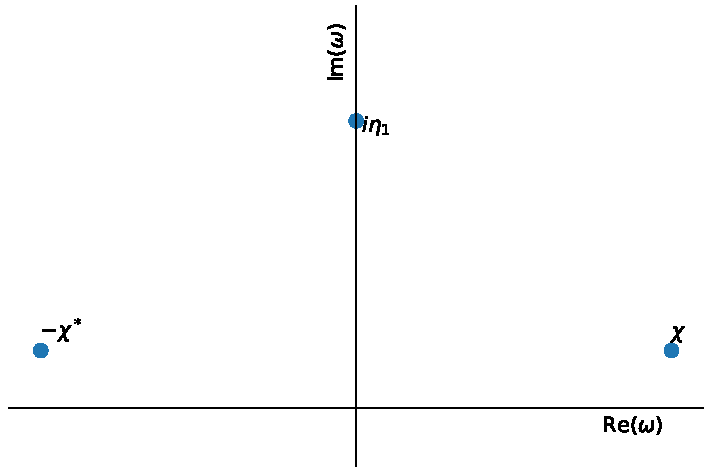
\includegraphics[width=0.5\textwidth]{F_poles}
	\caption{The pole structure of the Green's function of the non-Markovian Langevin equation with an exponential memory kernel.} 
	\label{fig:F_poles}
\end{figure*}

The Fourier spectrum of an exponential memory kernel is given by $\tilde{K}(\omega)=\frac{1}{1+i\omega\tau}$, which results in 3 poles in $\tilde{F}$ given by the zeros of the polynomial
\begin{equation}
	P(\omega) = i\tau\omega^3 + \omega^2 - i\omega(\omega_0^2\tau + \eta) - \omega_0^2.
\end{equation}
Since $P(i\omega)$ is a polynomial with real co-efficients, it follows from the complex conjugate root theorem that for any root $z$ of $P(\omega)$, $-z^*$ is also a root of $P(\omega)$. This allows us to make the ansatz that $P$ may be factorized as $P(\omega) = i\tau\left(\omega - \chi\right)\left(\omega + \chi^*\right)\left(\omega - i\eta_1\right)$ for some $\chi\in\mathbb{C}$ and ${\eta_1\in\mathbb{R}}$. While it is possible that $P(\omega)$ admits three imaginary solutions in some regions of the $\tau,\eta,\omega_0$ parameter space, these parameter ranges have not been encountered in our study of low-friction activated diffusion. If the Greens function $F(t)$ is to be causal, all three roots must occur in the upper half plane. We therefore find that the pole structure of $\tilde{F}(\omega)$ is of the form shown in Figure \ref{fig:F_poles}. A simple application of the residue theorem allows useful integrals of the form $\int\frac{dw}{2\pi} g\left(\omega\right) \left|\tilde{F}\left(\omega\right)\right|^2\Re(\tilde{K}(\omega))$ to be evaluated using the formula,
\begin{equation}
	\int\frac{dw}{2\pi} g\left(\omega\right) \left|\tilde{F}\left(\omega\right)\right|^2 \Re(\tilde{K}(\omega)) =  -\frac{1}{2 \tau^{2}}\left(\frac{1}{2 \chi' \chi''} \operatorname{Re}\left(\frac{g(\chi)}{\chi\left(\chi^{2}+\eta_{1}^{2}\right)}\right)+\frac{g(i\eta_{1})}{\left(|\chi|^{2}+n_{1}^{2}\right)^{2} \eta_{1}}\right), \label{eq:integral_over_CF}
\end{equation}
provided $g(\omega)$ is an entire function which decays sufficiently fast as $\operatorname{Im}({\omega})\rightarrow\infty$. In the formula above, $\chi'$ and $\chi''$ are defined as the real and imaginary components of $\chi$ respectively. Applied to the previously derived expressions of the ISF and kinetic energy autocorrelation function we obtain,

\begin{equation}
	ISF\left(\Delta \vec{K}, t\right) = ISF\left(\Delta \vec{K}, \infty\right) \exp\left(\frac{-\sigma^2\left|\Delta \vec{K}\right|^2}{2m^2\tau^2}\left(\frac{e^{-\chi''t}}{2\chi'\chi''}\operatorname{Re}\left(\frac{e^{i\chi't}}{\chi\left(\chi^2+\eta_1^2\right)}\right) + \frac{e^{-\eta_1t}}{\left(\left|\chi\right|^2+\eta_1^2\right)^2\eta_1}\right)\right) \label{eq:isf_exp}.
\end{equation}

\begin{equation}
	\left<E(0)E(t)\right>=\left<E(0)E(\infty)\right> + \frac{\sigma^4}{4\tau^4m^2}\left(\frac{e^{-\chi''t}}{2\chi'\chi''}\operatorname{Re}\left(\frac{\chi e^{i\chi't}}{\chi^2+\eta_1^2}\right) + \frac{\eta_1e^{-\eta_1 t}}{\left(\left|\chi\right|^2 + \eta_1^2\right)^2} \right)^2 \label{eq:ek_auto}
\end{equation}
\begin{equation}
	\left<E(0)E(\infty)\right> = \frac{\sigma^4}{4\tau^4m^2}\left(\frac{1}{2\chi'\chi''}\operatorname{Re}\left(\frac{\chi}{\chi^2+\eta_1^2}\right) - \frac{\eta_1}{\left(\left|\chi\right|^2 + \eta_1^2\right)^2} \right)^2.
\end{equation}
These expressions are extremely useful as the starting point for certain short-time theoretical calculations and for checking the correctness of computational work. The expression for $\left<E(0)E(\infty)\right>$ is particularly interesting as it is not immediately apparent that it is equal to $(k_BT)^2$. Nevertheless, numerically evaluating $\left<E(0)E(\infty)\right>/(k_BT)^2$ shows extremely small deviations from $1$, less than $10^{-12}$, likely due to numerical error.

\subsection{Energy exchange rate}

Although not a general proof, a careful expansion of the Green's function pole positions in small $\frac{\eta}{\tau}$ demonstrates that the second decay in Eq. \ref{eq:ek_auto} is suppressed by an additional factor of $\left(\frac{\eta}{\omega_0}\right)^2$ compared to the first. Therefore in the low friction limit, the kinetic auto-correlation function is approximately a single oscillating exponential decay with decay rate set by $2\chi''$. Since these two poles are present for all memory kernels (as discussed in Sec. \ref{sec:suppresion_factor}), this first decay is also present for all memory kernels. While more exotic memory kernels may have other decays which dominate the kinetic energy autocorrelation function, these may be numerically evaluated using Eq. \ref{eq:isf_exp} \& \ref{eq:ek_auto}, and we conject the effects are likely to remain small for small $\frac{\eta}{\omega_0}$. Although the total energy autocorrelation function has not been explicitly evaluated, simulated trajectories have shown that the decay rate of the total and kinetic energy autocorrelation functions is the same. We therefore conclude that the non-Markovian Langevin equation has an energy exchange rate in the low friction limit given by $\phi^{-1} = 2\chi''$. 

\end{document}
